\chapter{Софтуер за отдалечено управление}
\label{network_chapter}
\section{Формат на командите за отдалечено управление}
Отдалеченото управление се извършва посредством текстовите команди, описани в таблица \ref{tab:commands}. Командите се идентифирират по номер, когато се изпращат от клиента до сървъра, и по име, когато се въвеждат от команден ред или във файл. Командите, получени от сървъра, се изпращат към микроконтролера, където се записват в опашка и изпълняват.

\indent{}
Движението на робота се задава от командите MOV и MOVE, съответно за движение на един или на множество мотори. Команда MOV приема два параметъра - номер на мотор (виж таблица \ref{tab:addr_space}) и брой стъпки, които да изпълни. Команда MOVE приема шест параметъра - брой стъпки за изпълнение от всеки мотор, в нарастващ ред на номерата на моторите. Тази команда позволява едновременното движение на повече от един мотора. Отрицателен брой стъпки се използва за движение в обратна посока (виж таблица \ref{tab:addr_space}).\\
\indent{}
Команда OFF изключва захранването на мотора, чийто номер е подаден като параметър. За изключване на всички мотори се въвежда команда OFF със стойност на параметъра 6. Използва се когато е нужно ръчно преместване на механичните части на робота. Команда FREEZE поставя робота в режим на изчакване - прекратява изпълнението на опашката от команди. Команда OPTO се използва за засичане на предмети с оптичния сензорен хващач. Когато е изпратена команда OPTO с параметър 1 и по време на изпълнението на следващата MOV или MOVE команда бъде засечен предмет се прекратява текущата команда и се преминава към следваща. Команда OPTO с параметър 2 има същото поведение, с тази разлика, че командата за движение се прекратява, когато сензорът спре да засича предмет.
%Не питай...
\begin{table}[!htb]
    \centering
    \begin{tabular}{|c|c|p{147pt}|R{12mm}R{12mm}R{12mm}|}
        \hline
        \multirow{2}{*}{\textnumero} & \multirow{2}{*}{Име} & \centering\multirow{2}{*}{Пояснение} & \multicolumn{3}{c|}{Параметри}\\
        & & & \footnotesize{8} & \multicolumn{1}{|r|}{\footnotesize{16}} & \footnotesize{24}\\
        \hline
        \multirowcell{2}[0ex][c]{1} & \multirowcell{2}[0ex][c]{MOV} & Определен мотор извършва даден брой стъпки & \multirowcell{2}[0ex][c]{мотор} & \multicolumn{2}{|c|}{\multirowcell{2}[0ex]{стъпки}}\\
        \hline
        \multirow{2}{*}{2} & \multirow{2}{*}{MOVE} & \multirowcell{2}[0ex][l]{Всички мотори извършват\\ даден брой стъпки} & \multicolumn{2}{c|}{стъпки} &\\
        & & & \multicolumn{2}{c|}{x6} &\\
        \hline
        3 & OFF & Изключва определен мотор & \multicolumn{1}{c|}{мотор} & &\\
        \hline
        \multirow{2}{*}{4} & \multirow{2}{*}{OPEN\textunderscore FILE} & Изпълнява файл, записан на сървъра & \multicolumn{3}{c|}{\multirowcell{2}[0pt][c]{име на файла\\променлива дължина}}\\
        \hline
        \multirow{2}{*}{5} & \multirow{2}{*}{GOTO\textunderscore POS} & Запазена за бъдещо & \multicolumn{2}{c|}{позиция} &\\
        & & развитие & \multicolumn{2}{c|}{x6} &\\
        \hline
        \multirowcell{2}{6} & \multirowcell{2}[0pt][l]{GET\textunderscore POS} & Запазена за бъдещо & & &\\
        & & развитие & & &\\
        \hline
        \multirowcell{3}{7} & \multirowcell{3}{KILL} & \multirowcell{3}[0pt][l]{Аварийно спиране и\\изключване на всички\\мотори} & & &\\
        & & & & &\\
        & & & & &\\
        \hline
        \multirowcell{2}{8} & \multirowcell{2}{CLEAR} & Изчистване на опашката от команди & & &\\
        \hline
        \multirowcell{2}{9} & \multirowcell{2}{FREEZE} & Спира изпълнението на команди & & &\\
        \hline
        \multirowcell{2}{10} & \multirowcell{2}{RESUME} & Възобновява изпълнението на команди & & &\\
        \hline
        \multirowcell{2}{11} & \multirowcell{2}[0pt][l]{SAVE\textunderscore POS} & Запазена за бъдещо & & &\\
        & & развитие & & &\\
        \hline
        \multirowcell{3}{12} & \multirowcell{3}{OPTO} & Прекратяване на следващата команда, при сигнал от оптичния сензор & \multicolumn{1}{c|}{\multirowcell{3}{режим}} & &\\
        \hline
        \multirowcell{2}{13} & \multirowcell{2}{SET\textunderscore STEP} & Избор на движение с цяла стъпка или с полустъпка & \multicolumn{1}{c|}{\multirowcell{2}{стъпка}} & &\\
        \hline
        \multirowcell{2}{14} & \multirowcell{2}{SET\textunderscore SPEED} & Настройка на скоростта на стъпките & \multicolumn{1}{c|}{\multirowcell{2}{време}} & &\\
        \hline
    \end{tabular}
    \captionsetup{width=0.90\linewidth}
    \caption{Команди за отдалечено управление и техните параметри}
    \label{tab:commands}
\end{table}
Командата SET\textunderscore STEP променя режима на стъпка на моторите. Единственият й параметър има три валидни стойности: 0, 1 и 2. Те означават съответно: да се използва режимът, избран от SW1 (виж \ref{manual_cntrl_section}), полустъпка и пълна стъпка. Команда SET\textunderscore SPEED задава периода от време, който се изчаква след всяка стъпка. Параметърът й е времето в милисекунди или 0 за да се използва стойността, зададена чрез SW1.\\
\indent{}
Изброените до тук команди се записват в опашка в паметта на микроконтролера и се изпълняват в реда, в който са получени. Следващите команди са приоритетни - изпълняват се веднага при получаването им.\\
\indent{}
Такава команда е KILL. Използва се за аварийно изключване на робота. Не приема параметри, прекратява изпълнението на текущата команда и изключва всички мотори. Текущата команда не се изтрива и може да бъде възобновена. Команда RESUME също е приоритетна. Тя възобновява изпълнението на команди, спряно чрез FREEZE или KILL. Команда CLEAR изтрива цялата опашка от команди, включително и текущо изпълняваната команда.\\
\indent{}
Командата OPEN\textunderscore FILE е уникална с това, че не се изпълнява от микроконтролера, а от сървъра. Като параметър приема име на файл, чието съдържание да се изпрати от сървъра към микроконтролера. Файлът трябва да съдържа команди в описания тук формат. Ако файлът не се намира в папката, където е изпълнимия файл на сървъра, трябва към името на файла да се добави път спрямо тази папка.\\
\indent{}
Командите GOTO\textunderscore POS,  GET\textunderscore POS и SAVE\textunderscore POS са запазени за бъдещо развитие.
\section{Клиент}
Клиентската програма се използва от потребителя за изпращане на команди към сървъра. Състои се от файловете robko\textunderscore client.c, robko\textunderscore decode.c и съответните заглавни файлове. Програмата не разполага с графична среда и се изпълнява от команден ред. IP адреса на сървъра се подава като единствен параметър. На фигура \ref{fig:flch_client} е показана блок схема на програмата.
\begin{figure}[!htb]
    \centering
    \begin{tikzpicture}[node distance=1.5cm]
        \node (start) [startstop] {Начало};
        \node (addr_conv) [process, below of = start] {Преобразуване на адреса};
        \node (sock_open) [process, below of = addr_conv] {Отваряне на сокет};
        \node (cmd_in) [io, below of = sock_open] {Въвеждане на команда};
        \node (cmd_dec) [process, below of = cmd_in] {Декодиране на команда};
        \node (cmd_send) [io, below of = cmd_dec] {Изпращане на команда};
        \draw [arrow] (start) -- (addr_conv);
        \draw [arrow] (addr_conv) -- (sock_open);
        \draw [arrow] (sock_open) -- (cmd_in);
        \draw [arrow] (cmd_in) -- (cmd_dec);
        \draw [arrow] (cmd_dec) -- (cmd_send);
        \draw [arrow] (cmd_send) |- ([shift={(45mm,-5mm)}] cmd_send.south east) |- (cmd_in);
    \end{tikzpicture}
    \caption{Блок схема на клиентската програма}
    \label{fig:flch_client}
\end{figure}
\subsection{TCP сокет}
Програмата започва с преобразуване на IP адреса на сървъра от текстов низ към тип struct in\textunderscore addr. Отваря се TCP сокет към сървъра на порт 55321 чрез функцията connect(), предоставена от Berkeley sockets API. Файловият дескриптор на сокета се създава предварително от функцията socket(), а адресът и портът се задават от функцията bind().\\
\indent{}
Останалата част от алгоритъма се изпълнява в безкраен цикъл. Потребителят въвежда команда като текст в командния ред, разделяйки името на командата и параметрите с интервал. Програмата прочита въведения текстов низ от стандартния вход чрез функцията fgets(). Командата се декодира и изпраща по TCP сокета към сървъра с функцията write().
\subsection{Декодиране на команди}
\label{decode_section}
Декодирането на команди се извършва от функцията decode\textunderscore cmd(), дефинирана в robko\textunderscore decode.c. Приема два параметъра - указател към въведения от потребителя текстов низ и указател към началото на uint8\_t масив, в който се записва декодираната команда. Разпознаването на командата се извършва чрез последователно търсене на валидните имена на команди във въведения от потребителя низ чрез функцията strstr(). При съвпадение се извършват следващите стъпки. На нулева позиция в масива за декодирана команда се записва дължината на декодираната команда в байтове, включително байта за дължина. На първа позиция се записва номерът на командата. На следващите позиции се записват аргументите, ако има такива. Аргументите на някои команди са от тип int16\_t и заемат по две позиции от масива. Размерите на параметрите в битове са дадени в таблица \ref{tab:commands}. Преобразуването на параметрите от текст към целочислени типове се извършва от функцията strtol() и изрично конвертиране.
\section{Сървър}
Сървърната програма приема командите по TCP сокета и ги препраща към микроконтролера през сериен порт. При получаване на команда за изпълнение на файл прочита командите от съответния файл и ги изпраща към микроконтролера. Програмата се състои от файловете robko\_server.c, robko\_decode.c и съответните заглавни файлове. На фигура \ref{fig:flch_server} е показана блок-схема на програмата.
\begin{figure}[!htb]
    \centering
    \begin{tikzpicture}[node distance=1.75cm, text width=4cm]
        \node (start) [startstop] {Начало};
        \node (ser_init) [process, below of = start] {Инициализация на сериен порт};
        \node (sock_open) [process, below of = ser_init] {Отваряне на сокет};
        \node (wait) [process, below of = sock_open] {Изчакване};
        \node (cmd_in) [io, below of = wait] {Получаване на команда};
        \node (file_cond) [decision, below of = cmd_in, yshift = -1.75cm] {\makecell{Команда\\за отваряне\\на файл}};
        \node (cmd_resend1) [io, below of = file_cond, yshift = -2.25cm] {Препращане на командата през сериен порт};
        \node (eof) [decision, right of = file_cond, xshift = 4cm] {\makecell{Край на\\файла}};
        \node (read_cmd) [io, below of = eof, yshift = -2cm] {Прочитане на команда};
        \node (cmd_dec) [process, below of = read_cmd] {Декодиране на команда};
        \node (cmd_resend2) [io, below of = cmd_dec, yshift = -0.5cm] {Препращане на командата през сериен порт};
        \draw [arrow] (start) -- (ser_init);
        \draw [arrow] (ser_init) -- (sock_open);
        \draw [arrow] (sock_open) -- (wait);
        \draw [arrow] (wait) -- (cmd_in);
        \draw [arrow] (cmd_in) -- (file_cond);
        \draw [arrow] (file_cond) -- node [anchor = west] {Не} (cmd_resend1);
        \draw [arrow] (file_cond) -- node [anchor = south west] {Да} (eof);
        \draw [arrow] (eof) -- node [anchor = west] {Не} (read_cmd);
        \draw [arrow] (read_cmd) -- (cmd_dec);
        \draw [arrow] (cmd_dec) -- (cmd_resend2);
        \draw [arrow] (cmd_resend2.south) |- ([shift = {(27mm, -5mm)}] cmd_resend2.south east) |- ([shift = {(24mm, 20mm)}] eof.north east) -| (eof.north);
        \draw [arrow] (eof.east) -| node [anchor = south, shift = {(10mm, 0mm)}] {Да} ([shift = {(24mm, -10mm)}] cmd_resend2.south east) -| ([shift = {(-12mm, 0mm)}] file_cond.west) |- (wait);
        \draw [arrow] (cmd_resend1) -- ([shift = {(0mm, -47.5mm)}] cmd_resend1.south);
    \end{tikzpicture}
    \caption{Блок схема на сървърната програма}
    \label{fig:flch_server}
\end{figure}
\subsection{Серийна комуникация}
Сървърната програма използва библиотеката libserialport за комуникация с микроконтролера през сериен порт върху USB. Името на порта се избира чрез стойността на макроса SERIAL\_PORT във файла robko\_server.c. В началото на програмата серийният порт се инициализира и настройва със следните параметри: осембитова дума, проверка за четност (битът за четност е 1, ако в думата има четен брой единици), един стоп бит и скорост 115200 бода.
\subsection{TCP сокет}
Създаването на сокет се извършва както при клиента. Вместо функцията connect() се използва функцията listen(), която отваря сокета за заявки от страна на клиента. Функцията accept() изчаква клиентът да се свърже и когато го направи създава нов сокет през който да се обменят данните. Командите, изпращани от клиента, се приемат чрез функцията read().
\subsection{Препращане и изпълнение на команди}
Когато се получи команда се проверява дали е OPEN\_FILE. Ако е такава команда, се отваря съответния файл и една по една, командите от него се прочитат, декодират и изпращат към микроконтролера. За декодиране се използва същата функция, използвана и при клиента (виж \ref{decode_section}). Всички други команди директно се препращат. Първият байт от командата не се изпраща, а посочва дължината на командата в брой байтове. Причината при декодирането да се добавя дължината на командата в началото й е, че трябва да се знае колко байта трябва да бъдат изпратени по серийния порт. Не може да се предават данни до засичането на нулев байт, защото синтаксисът на командите позволява да се използват нулеви байтове в параметрите на командите.
\section{Наблюдение на TCP трафик}
Трафикът, обменян между клиента и сървъра, се наблюдава с програмата Wireshark. На фигура \ref{fig:TCP_session} са показани сегментите, съставящи TCP сесия за управление на РОБКО 01. Първите три сегмента изграждат сесията в съответствие с последователността на three-way handshake. Сегментите с четни номера от 4 до 14 включително съдържат команди, а сегментите с нечетни номера от 5 до 15 включително са потвърждения за успешно получаване на данни. Последните три сегмента завършват сесията.\\
\indent{}
Сегмент номер 6 е разгледан подробно на фигура \ref{fig:TCP_session}. Първият байт от данните показва, че сегментът съдържа общо 5 байта полезни данни. Вторият байт показва, че изпращаната команда е MOV (виж таблица \ref{tab:commands}). Първият параметър на командата е третия байт. От него става ясно, че командата се отнася за мотор номер 0. Последните два байта съставят втория параметър. Понеже сървърът и клиента се изпълняват на машини с little endian подредба на байтовете, първо се изпращат по-младшите байтове. В този пример вторият параметър има стойност 0x$0064 = 100_{(dec)}$ стъпки. 
\begin{figure}[!htb]
    \centering
    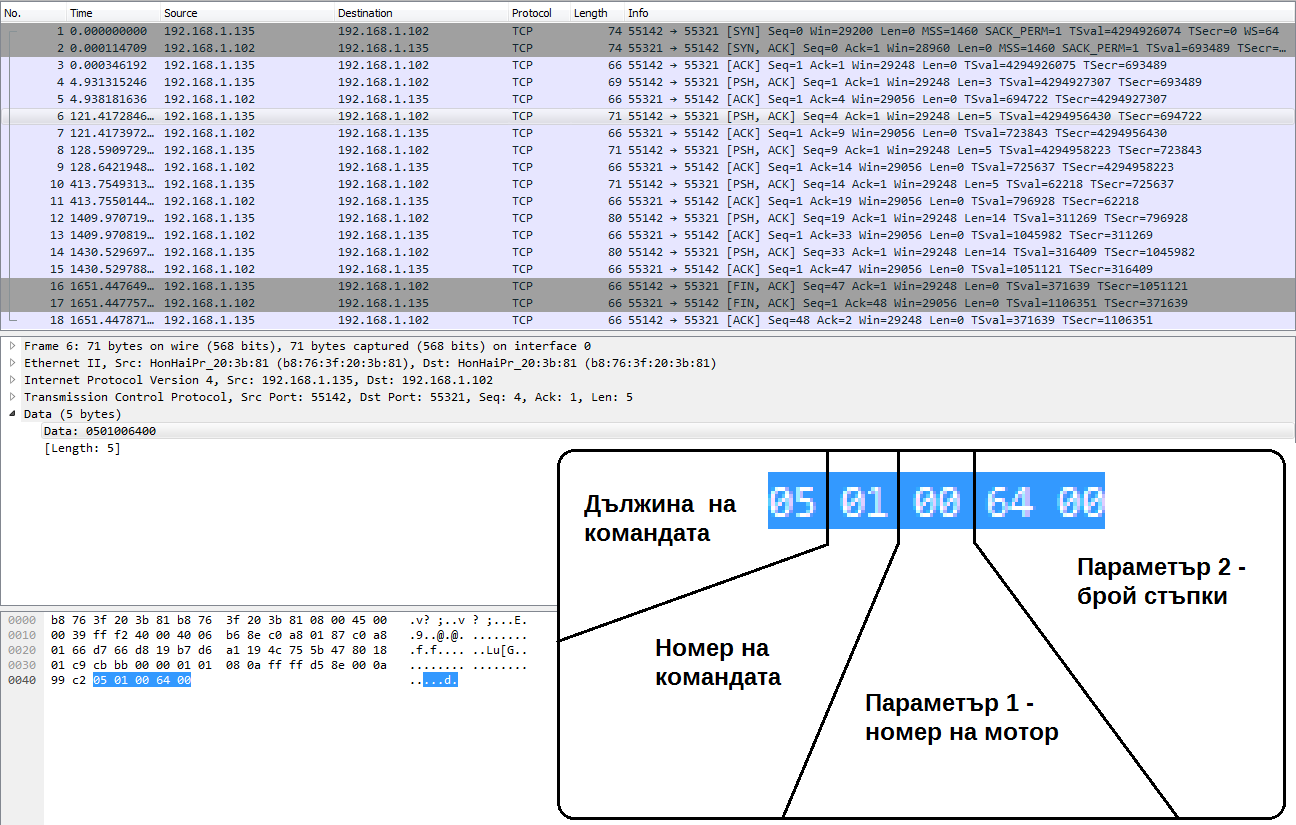
\includegraphics[width=\linewidth]{pictures/actual_packet.PNG}
    \caption{Примерна TCP сесия}
    \label{fig:TCP_session}
\end{figure}